%   システム情報工学演習第三 Antwort (2003/05/20) 
%
%                     by Masato ISHIKAWA : ishikawa@mei.titech.ac.jp
%
%                     2005/3/30  Modified by Hideaki Ishii 
%                     2007/10/11 Modified by Chiaki Kojima

%\documentclass[a4paper,10pt, twoside]{myarticle}
\documentclass[a4,10pt]{article}

\usepackage{amssymb,amsmath}
\usepackage{eclbkbox}
\usepackage{fancybox}
\usepackage[mathscr]{eucal}
% \usepackage[dvips]{color,graphicx}
\usepackage[dvipdfmx]{graphicx}
\usepackage{times}
%\usepackage{showkeys}
\usepackage{comment}


\textwidth 16.5cm
\oddsidemargin -0.2cm
\evensidemargin -0.8cm
\textheight 24.0cm
\topmargin -1.3cm

%\topmargin 2.4cm    % for PDF
\pagestyle{empty}


%
% Local preferences
%
\newcommand{\bmat}[1]{\left( \begin{array}{#1}}  	%begin matrix
\newcommand{\emat}{\end{array} \right)}			%end matrix
\newcommand{\pdf}[2]{\frac{\partial #1}{\partial #2}}
\newcommand{\df}[2]{\frac{d #1}{d #2}}
\newcommand{\Eu}{\mathbb{R}}

\newcounter{kadai}
\newenvironment{exercise}{%
  \addtocounter{kadai}{1} \vspace*{1.2ex}\par%
   {\noindent\bfseries [設問 \arabic{kadai}]}}  
       {\par%
\vspace*{1ex}}

\newcounter{jikken}
\newenvironment{experiment}{%
  \addtocounter{jikken}{1} \vspace*{1.2ex} \par%
   {\noindent\bfseries [実験 \arabic{jikken}]}}%
       {\par%
\vspace*{1ex}}

\newenvironment{exercise*}[1]{%
  \addtocounter{kadai}{1} \vspace*{1.2ex}\par%
   {\noindent\bfseries [課題 \arabic{section}.\arabic{kadai} #1]}}%

\newenvironment{prob}{%
  \vspace*{1.2ex}\par%
   {\noindent\bfseries 問:}}
       
{
%\newtheorem{definition}{Definition}
\newtheorem{proposition}{Proposition}
\newtheorem{theorem}{Theorem}
\newtheorem{example}{Example}
\newtheorem{remark}{Remark}
\newtheorem{corollary}{Corollary}
\newtheorem{lemma}{Lemma}
%\newtheorem{algorithm}{Algorithm}
\newtheorem{assumption}{Assumption}
\newtheorem{problem}{Problem}
\newtheorem{proof}{Proof}
  \renewcommand{\theproof}{} % *I* suppress numbering
  \renewcommand{\endproof}{{\hfill $\Box$}\break \hfil} 

\vspace*{1ex}}

%-------------------------------------------------------------------------
%
\begin{document}
\addtolength{\abovedisplayskip}{-.7mm}
\addtolength{\belowdisplayskip}{-.7mm}
\addtolength{\jot}{-.3mm}
\addtolength{\textfloatsep}{-2mm}
\addtolength{\floatsep}{2mm}
\addtolength{\baselineskip}{1.2mm}

%\vspace*{-15mm}

\begin{center}
 \LARGE \bfseries
 倒立振子の制御 ー マニュアル
\end{center}
%\begin{flushright}
%Version 09.10.01
%\end{flushright}



\section{今年の対応}
例年は本実験は倒立振子の実験機を用いて行っていたが,
今年は実験が行えないので配布するシミュレータを実験機の代替とし,
課題に取り組んでもらう. 

\section{準備}
\begin{enumerate}
    \item 各自のパソコンでMATLABを起動.この際,MATLABのバージョンを確認. 
    MATLABをインストールしていない場合は要相談.
    \item ダウンロードしたcartpend\_simulatorフォルダーをカレントフォルダーにする.
\end{enumerate}

% \section{実験で用いるソフトウェア}
% 本実験において用いるソフトウェアは,以下のとおりである.
% それぞれの特徴と基本的な使い方を簡単をまとめてあるので,必要に応じて読むこと.

\section{レポートについて}

\begin{enumerate}
    \item 実験のレポートは,テキスト中の全ての実験課題に対し考察を行い,全ての設問に対して解答すること.本マニュアルの\textbf{問}はボーナス課題とする.
    積極的に取り組んでください.
    \item 図はpng形式やjpg形式で保存してレポートに貼ること.
    スクリーンキャプチャでも良いが,画質は落ちる.
% なお,テキストや他の人のレポートを一部でも写して提出した場合には,「倒立振子の制 御」の成績を不合格とします.
\end{enumerate}

\subsection*{連絡先}
\begin{itemize}
    \item 担当:山内淳矢 助教
    \item メールアドレス:junya\_yamauchi \_at\_ ipc.i.u-tokyo.ac.jp(\_at\_を@に置き換える)
    \item 内線:26890
\end{itemize}

\begin{figure}[h]
 \centering 
 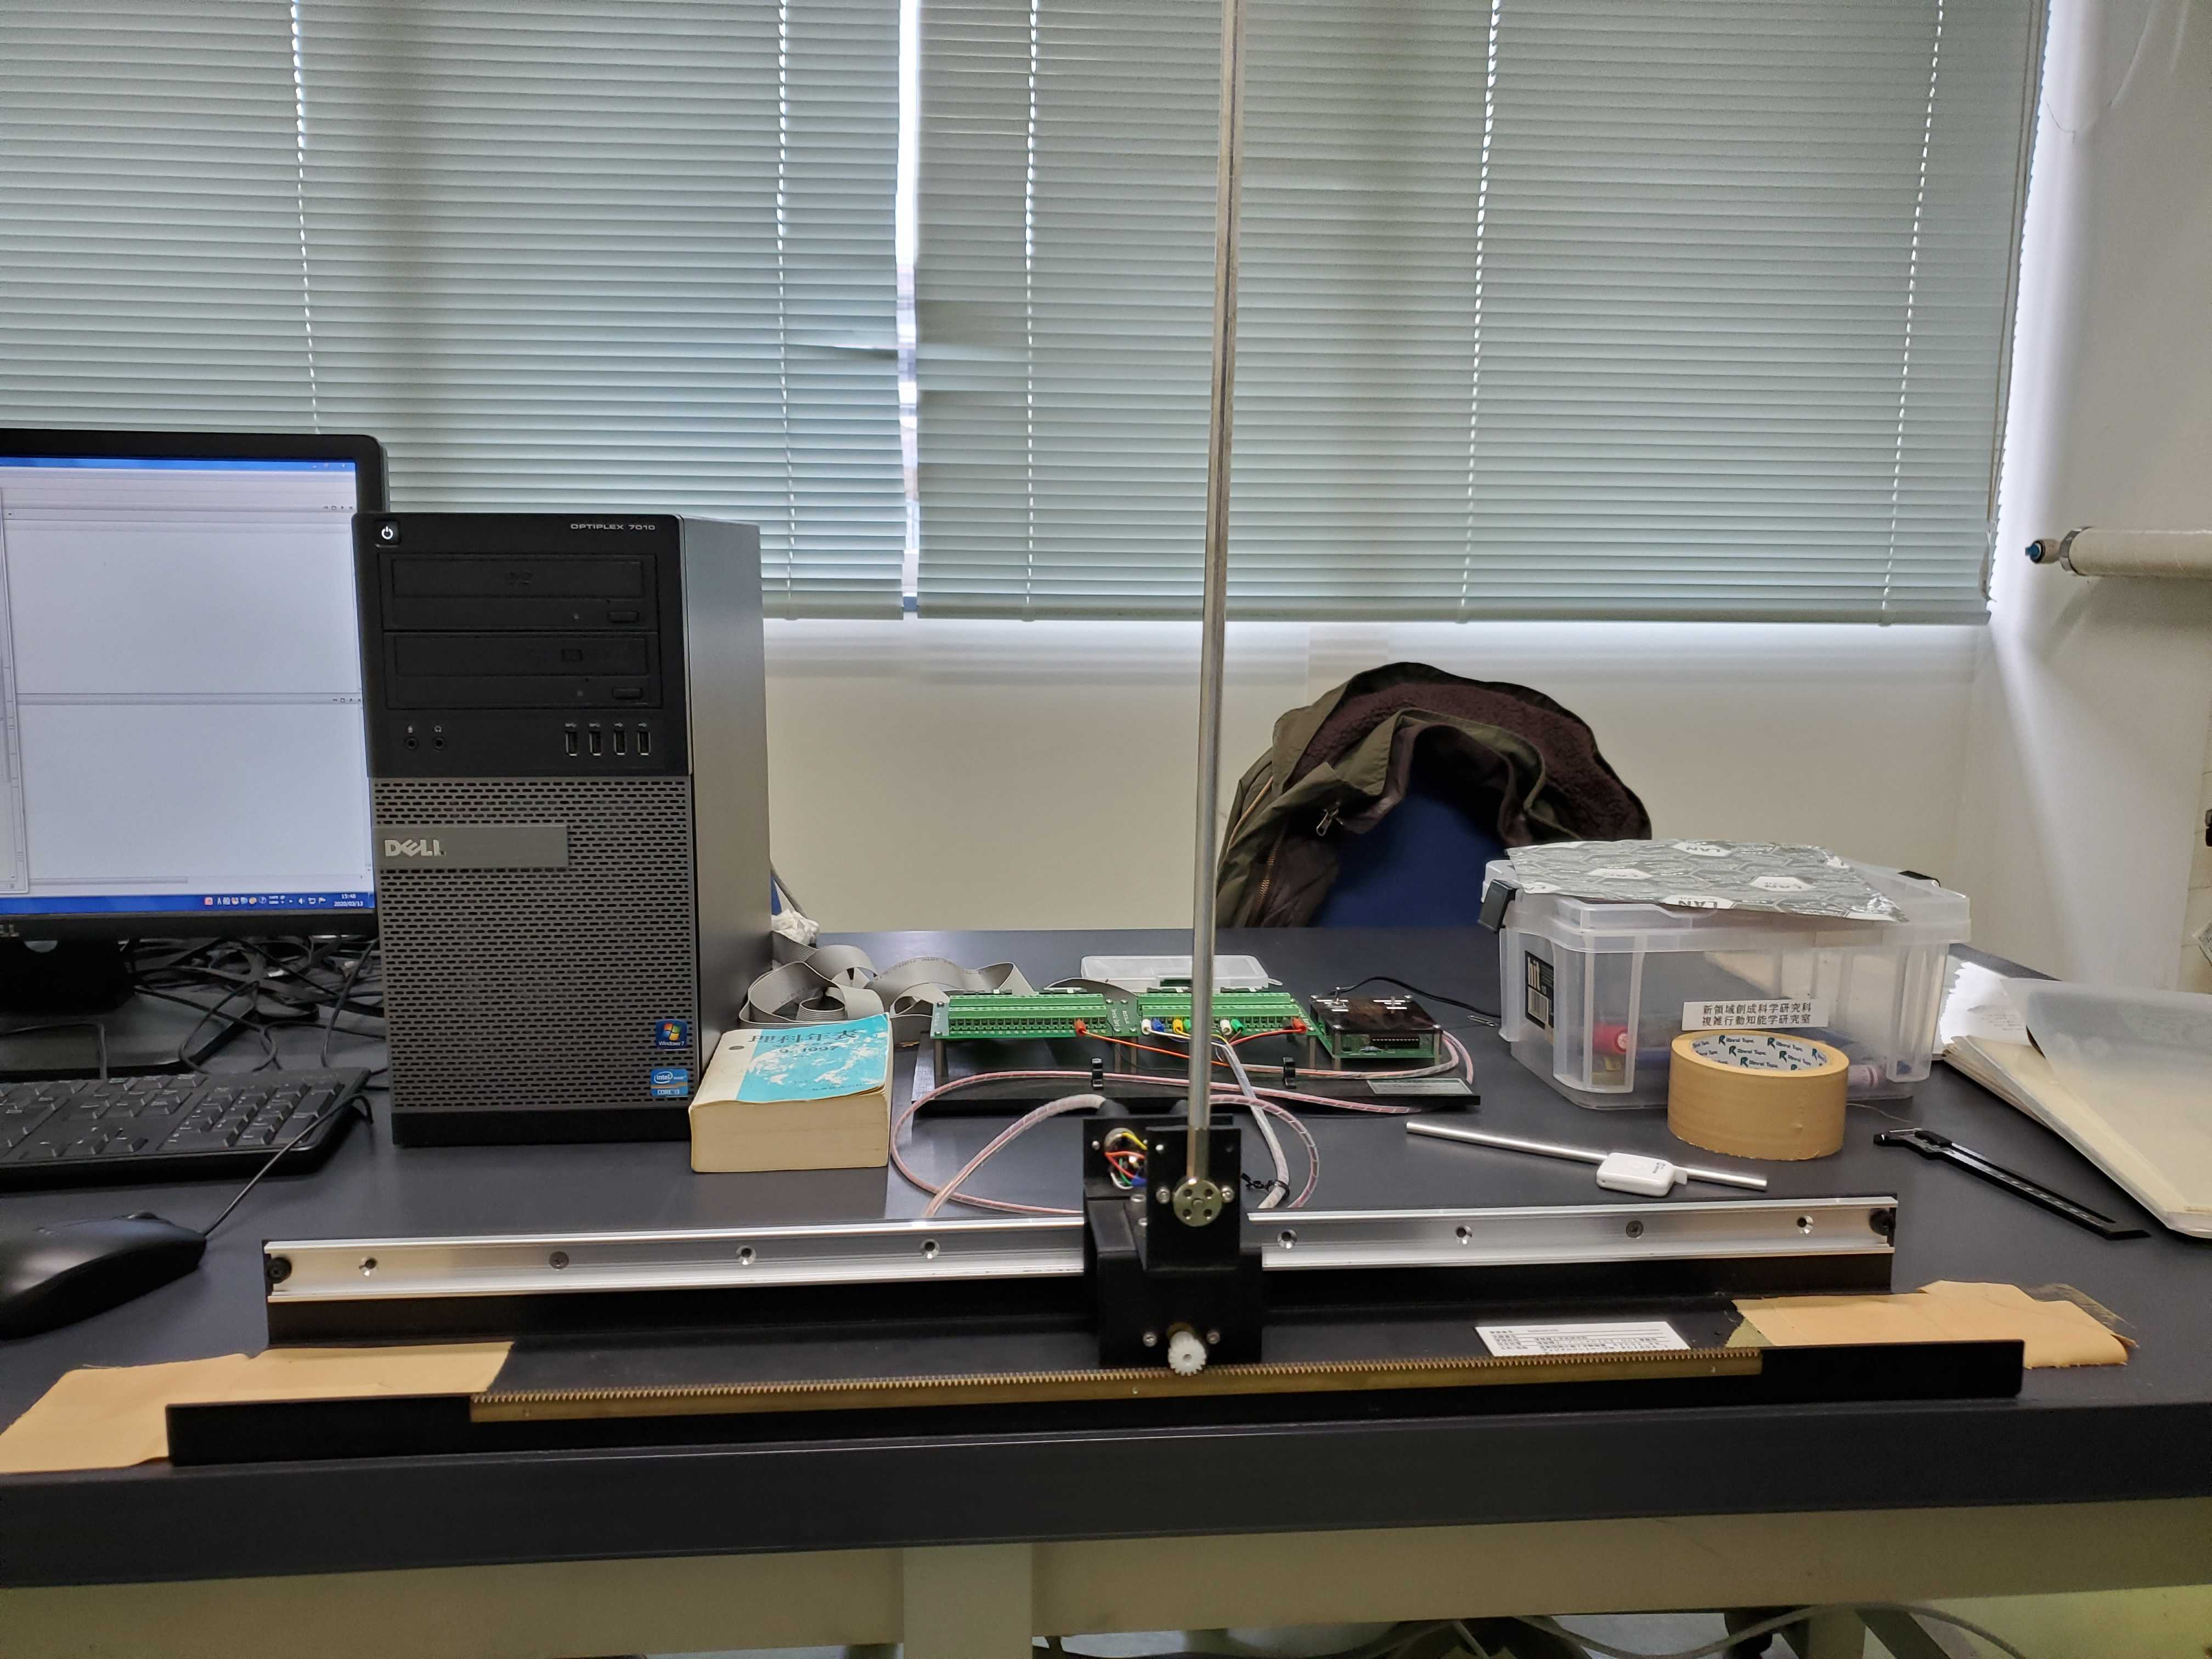
\includegraphics[height=7cm]{figs/cart_pend.jpg}
\end{figure}

\begin{center}
 \LARGE \bfseries 倒立振子の制御 ー 台車パラメータ同定
\end{center}

\begin{enumerate}
    \item cart\_identification.mを開く.
    
    \item matlab versionのセクション,パラメータmatlabversionに
    自分の使っているMATLABのバージョンを設定.
    MATLAB 2019aかMATLAB 2019bを使っている場合は2019を設定し,
    MATLAB 2018aかMATLAB 2018bの場合は2018に設定.
    MATLAB 2020aを使っている場合は2020に設定.

    \item ステップ入力の電圧値であるパラメータ$E$を$1.1$V〜$1.7$Vの間で変更する.
    \item  実行ボタンを押してシミュレータを実行する.
    1秒後に台車が右側へと移動し,2秒後に停止する.
    台車の停止後に台車の位置と入力電圧の結果が表示される.
    \item テキストに書いてある方法に従って,$M$と$\hat{D}_x$を求める.
    \item レポート用に図を保存する.
    「ファイル」 → 「名前を付けて保存」 → 「ファイル名」は適当に設定し, 「ファイルの種類」をpngかjpgに設定して保存.
    特に保存先を指定しなければカレントフォルダー(つまりcartpend\_simulator)に保存される.
\end{enumerate}


\newpage

\begin{center}
 \LARGE \bfseries 倒立振子の制御 ー 振子パラメータ同定
\end{center}

\begin{enumerate}
    \item pend\_identification.mを開く.
    
    \item MATLABのバージョンを設定.

    \item parameter settingのセクションで,パラメータtheta\_initを設定し,実行する.
    単位がradianであることに注意する.
    $\theta = 0$で上向き,$\theta = \pi$で下向き.
    
    必要に応じて,set\_paramで設定されているパラーメータStopTimeを調整することで,シミュレーションの時間を調整すること.
    
    % \item Simulinkのメニューの「ターゲットに接続」のアイコンをクリックし,次にメニューの「リア ルタイムコードを開始」のアイコン(右向きの三角形)をクリックする.
    % その直後に振子を適 当な角度まで持ち上げ放す(クリックした時点での振子の角度が原点になるので,
    % 持ち上げるタイミングに注意する).
    % 10秒後に停止し,その後に``Pend(振子の角度)'' の画面が現れる.

    \begin{prob}
    どの程度大きな角度で振動させるのがよいか?(ヒント:用いた振子のモデルは線形化したものである)
    \end{prob}

    \item  テキストに書いてある方法に従って,$I$と$D_\theta$を導出する.
    
    \item レポート用に図を保存する.
    「ファイル」 → 「名前を付けて保存」 → 「ファイル名」は適当に設定し, 「ファイルの種類」をpngかjpgに設定して保存.
    特に保存先を指定しなければカレントフォルダー(つまりcartpend\_simulator)に保存される.
    
    振子の挙動のラプラス変換は,テキスト中 (12) 式の2次系として表される.
    これを2次系の標準的な形で書くと
    \begin{align*}
        \Theta(s) = \frac{K\omega_n}{s^2 + 2 \zeta \omega_n s + \omega_n^2}
    \end{align*}
    となる.
    ただし$\omega_n$は自然角振動数,$\zeta$は減衰係数,$K$は適当な実数で系の初期値により決まる.
    これを逆ラプラス変換すると,
    \begin{align} \label{eq:theta}
        \theta(t) = \frac{K\omega_n}{\sqrt{1-\zeta^2}} e^{- \zeta \omega_n t} 
        \sin(\omega_n \sqrt{1-\zeta^2} t)
    \end{align}
    となる.
    明らかにこの応答の周期$T$は    
    \begin{align} \label{eq:T}
        T = \frac{2\pi}{\omega_n \sqrt{1-\zeta^2}} 
    \end{align}
    である.
    また$\theta(t)$がピーク値をとる時間を$t_0, ~ t_1,~ t_2, \ldots$と表し,一周期あたりのピークの減衰比を$\lambda:= \dfrac{\theta(t_{i+2})}{\theta(t_{i})}$とする.
    このとき,(\ref{eq:theta})式から
    \begin{align} \label{eq:lambda}
        \lambda = e^{-\zeta \omega_n T}.
    \end{align}
    
    \begin{prob}
        上記(\ref{eq:T})の周期$T$はどのように求められるか?
    \end{prob}
    
    実測値から$T$と$\lambda$を求め,上の(\ref{eq:T})式と(\ref{eq:lambda})式を用いて,
    $\zeta$と$\omega_n$の組を求めよ.
    最後にテキスト(14)式の自然角振動数と減衰係数の式などから$I$と$D_\theta$を求める.
\end{enumerate}

\newpage

\begin{center}
 \LARGE \bfseries 倒立振子の制御 ー 状態フィードバック則の設計
\end{center}

\subsection*{極配置法}
\begin{enumerate}
    \item cartpend\_PoleAssignment.mを開く.
    
    \item MATLABのバージョンを設定.

    \item  台車と振子の同定結果をもとに,テキスト中 (5) 式の状態方程式における行列 $A$,$B$を求める.
    
    % \item Simulinkのメニューの「ターゲットに接続」のアイコンをクリックし,次にメニューの「リア ルタイムコードを開始」のアイコン(右向きの三角形)をクリックする.
    % その直後に振子を適 当な角度まで持ち上げ放す(クリックした時点での振子の角度が原点になるので,
    % 持ち上げるタイミングに注意する).
    % 10秒後に停止し,その後に``Pend(振子の角度)'' の画面が現れる.

    \item  配置したい閉ループ系の極$p_1,~ p_2,~ p_3,~ p_4$ の値を,cartpend\_PoleAssignment.mに入力する.
    
    \item  初期値position\_initとtheta\_initを入力する.
    
    \item cartpend\_PoleAssignment.mを実行する.
    このとき,コマンドplaceによりコントローラのゲイン$F$が計算される.
    さらに,各状態の応答が表示される.
    必要に応じて,set\_paramで設定されているパラーメータStopTimeを調整することで,シミュレーションの時間を調整すること.
    
    $(A,B)$が可制御対であるとき,ある正則
    行列$T$が存在して
    \begin{displaymath}
     \bar{A} = T^{-1}AT = \bmat{cccc} 
                  0 & 1 & 0 & 0 \\
                  0 & 0 & 1 & 0 \\
                  0 & 0 & 0 & 1 \\
                  -\alpha_0 & -\alpha_1 & -\alpha_2 & -\alpha_3 
               \emat, \quad
     \bar{B} = T^{-1}B = \bmat{c} 0 \\ 0 \\ 0 \\ 1 \emat
    \end{displaymath}
    が成立する.
    ただし,$\alpha_0, \ldots, \alpha_3$は$\bar{A}$と$A$の特性多項式
    \begin{equation*}
    \left|s I-\bar{A}\right|=s^4 + \alpha_3s^3 + \alpha_2s^2 + \alpha_1s + 
     \alpha_0.  
    \end{equation*}
    の係数である.
    つぎに,
    指定された固有値を$p_1,\cdots,p_4$とする.
    対応する閉ループ系の特性多項式を考えて
\begin{displaymath}
 (s-p_1)(s-p_2)(s-p_3)(s-p_4) = s^4 + \gamma_3 s^3 + \gamma_2 s^2 + \gamma_1 s^1 + \gamma_0
\end{displaymath}
となるように右辺の係数$\gamma_0,\cdots,\gamma_3$を定める.
    このとき,
    \begin{align}
         \bar{F}=\bmat{cccc} \alpha_0-\gamma_0 & \alpha_1-\gamma_1 & \alpha_2-\gamma_2 & \alpha_3-\gamma_3 \emat 
    \end{align}
   とおき,さらに$F$を
   \begin{align}
       F = \bar{F}T^{-1}
   \end{align}
    によって定める.
    すると,
    \begin{align}
        A+BF = T(\bar{A}+\bar{B}\bar{F})T^{-1}
    \end{align}
    であり,さらに
    \begin{align}
         \bar{A}+\bar{B}\bar{F} = 
         \bmat{cccc} 
                  0 & 1 & 0 & 0 \\
                  0 & 0 & 1 & 0 \\
                  0 & 0 & 0 & 1 \\
                  -\gamma_0 & -\gamma_1 & -\gamma_2 & -\gamma_3 
               \emat
    \end{align}
    となるから,$A+BF$の特性多項式は
    \begin{align}
        \left|s I-(A+BF)\right|&=s^4 + \gamma_3s^3 + \gamma_2s^2 + \gamma_1s + 
        \gamma_0 \\
        &= (s-p_1)(s-p_2)(s-p_3)(s-p_4)
    \end{align}
    となる.
    つまり,$F$により閉ループ系の
    極を指定された$p_1,~ p_2, ~ p_3, ~ p_4$に設定することができた.
    
    \item レポート用に図をpngかjpg形式で保存.
    
    
    \begin{prob}
        極の選び方とシステムの応答の間には,どのような関係があるだろうか?
    \end{prob}
    
    \begin{prob}
        実験では制御入力は一定値以上にすることができない.
        これは制御設計をする上で,どのように考慮すべきか?
    \end{prob}
    
   \begin{prob}
        simulationセクションのパラメータhuman\_inputを1に設定して倒立振子系に外乱を与えたとき,極の設定はその挙動にどのように影響するか?
    \end{prob}

\end{enumerate}



\subsection*{最適レギュレータ}
\begin{enumerate}
    \item cartpend\_OptimalRegulator.mを開く.
    
    \item MATLABのバージョンを設定.

    \item  台車と振子の同定結果をもとに,テキスト中 (5) 式の状態方程式における行列 $A$,$B$を求める.

    \item  重み行列$Q$と$R$を選ぶ.
    簡単のために,最初は$Q$を対角行列とするとよい.
    
    \item  初期値position\_initとtheta\_initを入力する.
    
    \item cartpend\_OptimalRegulator.mを実行する.
    このとき,コマンドlqrによりコントローラのゲイン$F$が計算される.
    さらに,各状態の応答が表示される.
    必要に応じて,set\_paramで設定されているパラーメータStopTimeを調整することで,シミュレーションの時間を調整すること.
    
    \item レポート用に図をpngかjpg形式で保存.
   
   \begin{prob}
        行列$Q$と$R$の選び方は,システムの応答にどのように影響するか?
    \end{prob}
    
   \begin{prob}
        simulationセクションのパラメータhuman\_inputを1に設定して倒立振子系に外乱を与えたとき,$Q$と$R$の設定はその挙動にどのように影響するか?
    \end{prob}
   
\end{enumerate}

\newpage 

\begin{center}
 \LARGE \bfseries 倒立振子の制御 ー オブザーバを用いた状態フィードバック則の設計
\end{center}

\subsection*{オブザーバの設計}
\begin{enumerate}
    \item cartpend\_Observer.mを開く.
    
    \item MATLABのバージョンを設定.

    \item  台車と振子の同定結果をもとに,テキスト中 (5) 式の状態方程式における行列 $A$,$B$を求める.
    
    % \item Simulinkのメニューの「ターゲットに接続」のアイコンをクリックし,次にメニューの「リア ルタイムコードを開始」のアイコン(右向きの三角形)をクリックする.
    % その直後に振子を適 当な角度まで持ち上げ放す(クリックした時点での振子の角度が原点になるので,
    % 持ち上げるタイミングに注意する).
    % 10秒後に停止し,その後に``Pend(振子の角度)'' の画面が現れる.

    \item  極配置法か最適レギュレータによりオブザーバゲイン$L$を設計する.
    
    \item cartpend\_Observer.mを実行する.
    
    オブザーバゲイン$L$の設計問題は,状態フィードバック則の設計問題と以下の意味で{\bfseries 双対}となっている.
     $A+LC$に任意の実軸対称な固有値を配置できるための必要十分条件は,$(A,C)$が可観測であることである.
    この条件は,$(A^T, C^T)$が可制御であることと等価である.
    つまり,別のシステム
    \begin{align*}
        \dot{x} &= A^Tx + C^Tu \\
        y &= B^Tx
    \end{align*}
    が可制御であることと,テキスト中 (5) 式のシステムが
    可観測であることは等価である.
    したがって,
    $(A^T,C^T)$に対して極配置法を実行することによって$L^T$が設計できる.
    
    % \item レポート用に図をpngかjpg形式で保存.
    
    \begin{prob}
        振子が倒立していないとき,状態の推定が
        うまくいかないのはなぜか考察せよ.
    \end{prob}
    
\end{enumerate}    
    
\subsection*{極配置法}
\begin{enumerate}
    \item cartpend\_obs\_PoleAssignment.mを開く.
    
    \item MATLABのバージョンを設定.

    \item  台車と振子の同定結果をもとに,テキスト中 (5) 式の状態方程式における行列 $A$,$B$を求める.
    
    % \item Simulinkのメニューの「ターゲットに接続」のアイコンをクリックし,次にメニューの「リア ルタイムコードを開始」のアイコン(右向きの三角形)をクリックする.
    % その直後に振子を適 当な角度まで持ち上げ放す(クリックした時点での振子の角度が原点になるので,
    % 持ち上げるタイミングに注意する).
    % 10秒後に停止し,その後に``Pend(振子の角度)'' の画面が現れる.

    \item  配置したい閉ループ系の極$p_{11},~ p_{12},~ p_{13},~ p_{14}$および$p_{21},~ p_{22},~ p_{23},~ p_{24}$の値を,cartpend\_obs\_PoleAssignment.mに入力する.
    
    \item  初期値position\_initとtheta\_initを入力する.
    
    \item cartpend\_obs\_PoleAssignment.mを実行する.
    このとき,コマンドplaceによりコントローラのゲイン$F$とオブザーバのゲイン$L$が計算される.
    さらに,各状態の応答が表示される.
    必要に応じて,set\_paramで設定されているパラーメータStopTimeを調整することで,シミュレーションの時間を調整すること.
    
    \item レポート用に図をpngかjpg形式で保存.
    
    
%     \begin{prob}
%         極の選び方とシステムの応答の間には,どのような関係があるだろうか?
%     \end{prob}
    
%   \begin{prob}
%         simulationセクションのパラメータhuman\_inputを1に設定して倒立振子系に外乱を与えたとき,極の設定はその挙動にどのように影響するか?
%     \end{prob}

\end{enumerate}



\subsection*{最適レギュレータ}
\begin{enumerate}
    \item cartpend\_obs\_OptimalRegulator.mを開く.
    
    \item MATLABのバージョンを設定.

    \item  台車と振子の同定結果をもとに,テキスト中 (5) 式の状態方程式における行列 $A$,$B$を求める.

    \item  重み行列$Q_1$,$R_1$および$Q_2$,$R_2$を選ぶ.
    
    \item  初期値position\_initとtheta\_initを入力する.
    
    \item cartpend\_obs\_OptimalRegulator.mを実行する.
    このとき,コマンドlqrによりコントローラのゲイン$F$とオブザーバのゲイン$L$が計算される.
    さらに,各状態の応答が表示される.
    必要に応じて,set\_paramで設定されているパラーメータStopTimeを調整することで,シミュレーションの時間を調整すること.
    
    \item レポート用に図をpngかjpg形式で保存.
   
%   \begin{prob}
%         行列$Q$と$R$の選び方は,システムの応答にどのように影響するか?
%     \end{prob}
    
%   \begin{prob}
%         simulationセクションのパラメータhuman\_inputを1に設定して倒立振子系に外乱を与えたとき,$Q$と$R$の設定はその挙動にどのように影響するか?
%     \end{prob}
   

\end{enumerate}


\end{document}
